\section{Results and robot-specific discussions} \label{sec:results}

This chapter presents and discusses the results of the tests with \FixRob and \TurnRob. The robots were tested under controlled conditions described in Section \ref{sec:data_collection}. The main focus of this chapter is analysing and discussing the robot-specific benchmarks in terms of speed, intersection navigation, power consumption and cost. The raw data of the measurements and the analysis tables can be found on GitHub\footnote{\url{https://github.com/marvinknoll/nxt_maze_solving/tree/main/benchmarks}}.

\subsection{Fixed-sensor robot}

\subsubsection{Results} \label{sec:fixed_results}
Table \ref{tab:one_fixed_results} summarises the key statistics for the eleven runs of the robot configuration with a single fixed sensor. On average, the complete runs took 334.77 seconds and had a relatively low standard deviation of 9.4 seconds. The most time was spent at intersections, with an average of 243.17 seconds, while the least time was spent on realignments, at 34.39 seconds on average. The standard deviations of the measured times show that the time spent on the line was the most constant, while the time spent realigning was the least constant. The average voltage difference of the battery before and after the test runs was 57.55 millivolts.

\begin{table}[h!]
\caption{\FixedSensorRobot~- Summary of key statistics}
\label{tab:one_fixed_results}
\resizebox{\textwidth}{!}{
\begin{tabular}{lllllll}
\hline
                   & \multicolumn{4}{c}{Time {[}s{]}}                   & \multicolumn{1}{l}{} & \multicolumn{1}{l}{}    \\ \cline{2-5}
                   & Total   & Intersections & Black lines & Realignments & \#Realignments       & Voltage difference {[}mV{]} \\ \hline
Average            & 334.77  & 243.17       & 57.21      & 34.39        & 26.18                & 57.55                   \\
Sum                & 3682.45 & 2674.83      & 629.31     & 378.31       & 288                  & 633                     \\
Minimum            & 323.083 & 239.66       & 56.07      & 23.09        & 17                   & 5                       \\
Maximum            & 350.168 & 245.18       & 58.27      & 49.43        & 32                   & 136                     \\
Standard Deviation & 9.49838 & 1.85923      & 0.65651    & 8.27200      & 3.97034              & 36.0398                 \\ \hline
\end{tabular}
}

\end{table}


Figure \ref{fig:fixed-power} shows the battery voltage before and after each of the eleven runs, indicating the robot's power consumption. 

\begin{figure}[h!]
    \centering
    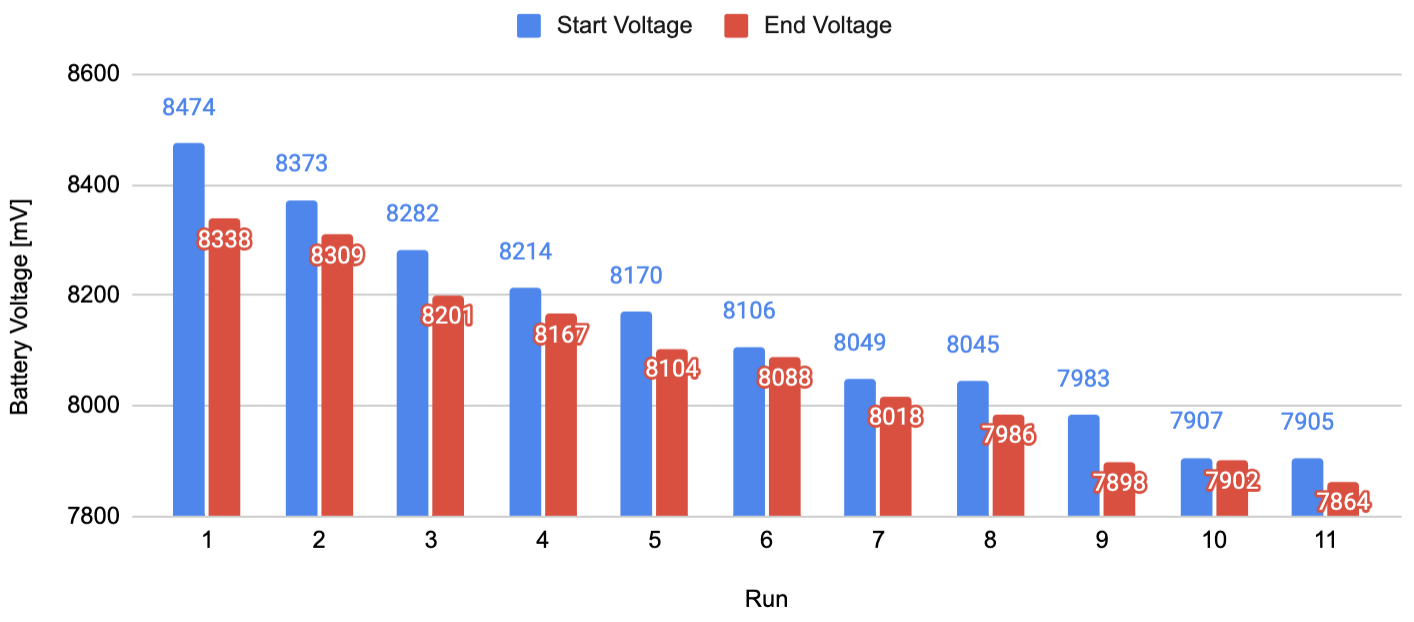
\includegraphics[width=\textwidth]{resources/fixed-power.png}
    \caption{\FixRob~- Comparison of start and end battery voltage per run}
    \label{fig:fixed-power}
\end{figure}

Figure \ref{fig:fixed-intersection-times} shows the average time that the robot required to complete the individual intersection types described in Figure \ref{fig:intersection_types}. Dead ends, with an average of 22.7 seconds, took the robot the longest to scan and navigate. In contrast, “left \& straight”, “left \& straight \& right”, “left”, and “left \& right” intersections took the least time with averages between 10.87 and 11.03 seconds.

\begin{figure}[hbt!]
    \centering
    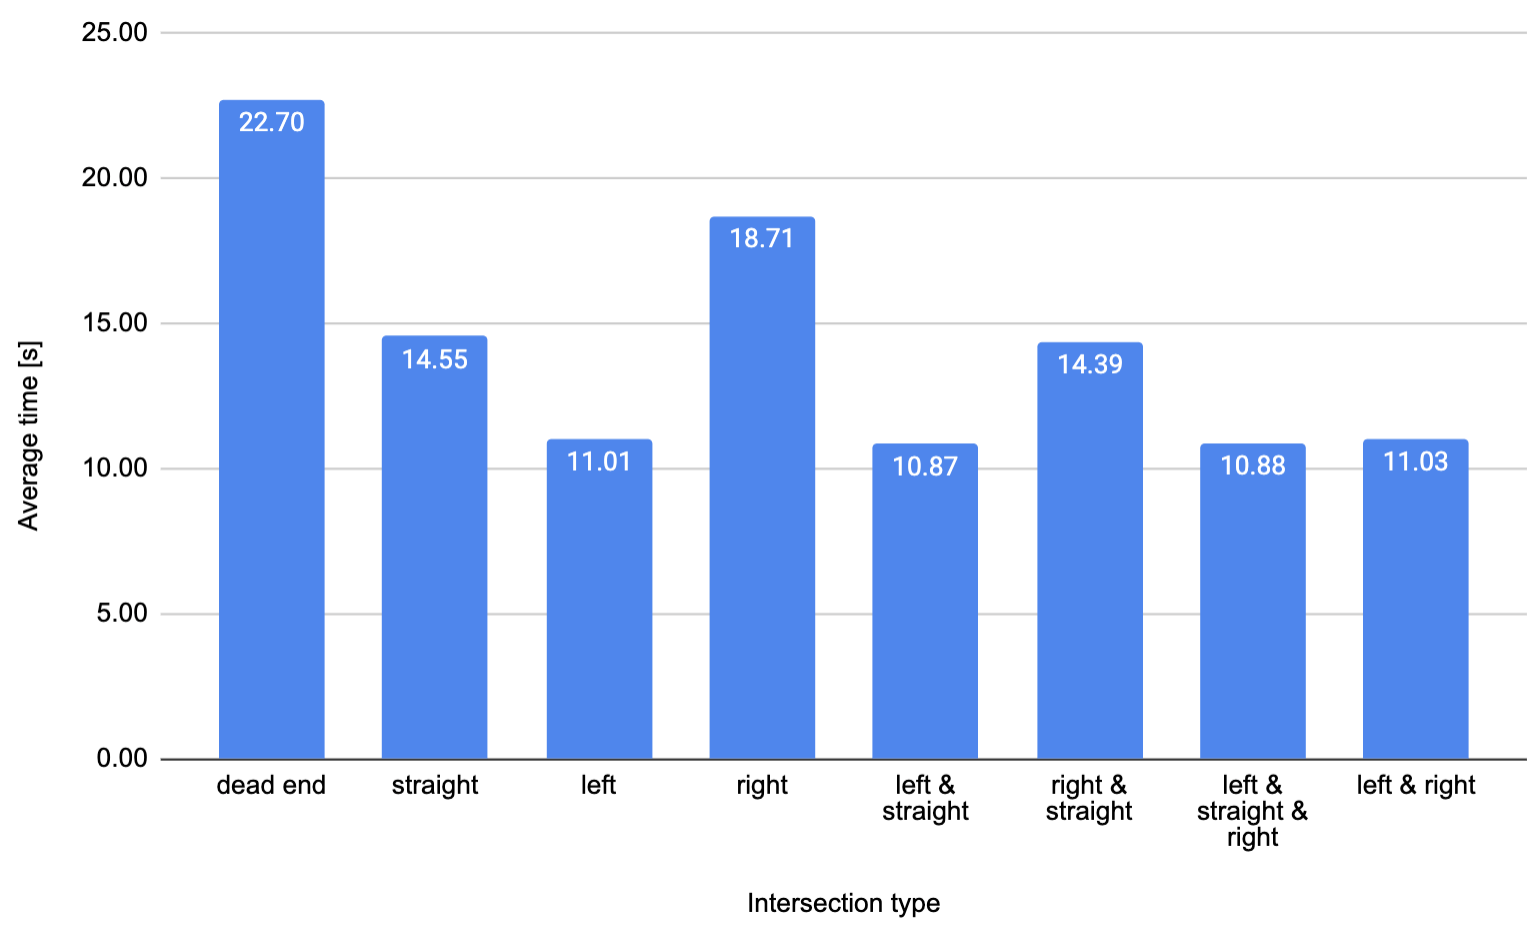
\includegraphics[width=\textwidth]{resources/fixed-intersection-times.png}
    \caption{\FixRob~- Average time per intersection type}
    \label{fig:fixed-intersection-times}
\end{figure}

\subsubsection{Discussion} \label{sec:fixed_discussion}
The standard deviation of 9.498 for the total run duration indicates the consistent performance of the robot. From the standard deviation of 8.272, it becomes clear that the time for realignment is the least consistent one. These deviations are understandable because the robot has only one sensor and therefore does not know in which direction to reorient itself to find the line. Although the robot tries to make an educated guess about which direction to scan first, it sometimes scans in the wrong direction, resulting in a higher standard deviation.

The collected data allowed for calculating the time the robot spent exclusively on the line. This was done by adding the time spans between intersection scans and realignments. The granular time measurements also allowed for calculating the time spent between two specific intersections. It was found that the time between the last intersection (\#13) and the end of the maze (\#14) averaged 13 seconds, while all other lines between two intersections averaged only 2.57 seconds. This difference is present because the detection of the end of the maze is relatively slow, and the timing stops only after the end has been detected and the driving motors are still.

The high standard deviation of 36.04 in the battery voltage data  and the fact that successive runs' end and start voltages differ from each other suggest significant measurement inaccuracies. It is not fully clear why the measurements are so inconsistent. However, it is known that factors such as temperature or start voltage can strongly influence the measured voltage. Another factor which makes it harder to measure the battery voltage is that the voltage of NiMH batteries can vary significantly during discharge. Finally, it is also possible that the NXT brick is inaccurate in measuring the battery voltage.

The data in Figure \ref{fig:fixed-intersection-times} show the average time spent at the different intersection types. In the chart, four groups of intersection types with similar times can be identified. The group elements have in common which direction the robot finally takes at the intersection.

An interesting observation is that \textit{right} turns take longer than \textit{left} turns. This is because the robot turns 135 degrees counterclockwise to find a possible \textit{left} path, and when it finds it, it takes it. Also, for a \textit{right} turn, it first rotates 135 degrees counterclockwise to ensure no \textit{left} path is available and then must rotate 225 degrees clockwise to align with the \textit{right} path, which takes more time.

The most time was required for \textit{dead ends}, which makes sense since the robot needs to turn the farthest to scan and navigate such intersections. As Section \ref{sec:fixed_intersection_scan} describes, the robot turns 135 degrees counterclockwise to ensure there is no \textit{left} or \textit{straight} path available and then 315 degrees clockwise to check the availability of the \textit{right} path and, finally, head back as it is a \textit{dead end}.

In summary, the results have shown that the robot requires the least time for the highest priority turn of \textit{left}. For the remaining turns, \textit{straight}, \textit{right}, and \textit{back}, more and more time is required in descending order of priority.

The cost of the robot is the bare minimum for a line-following robot built with LEGO Mindstorms, as all the electronic parts are necessary. However, what could undoubtedly be reduced are the remaining parts that make up the robot.

\subsection{Turning-sensor robot}

\subsubsection{Results} \label{sec:turning_results}

Table \ref{tab:one_turning_results} presents the critical statistics for the robot configuration with a single turning sensor. On average, this robot took 333.3 seconds to complete a single run with a relatively low standard deviation of 9.28775. The average time spent scanning and navigating intersections was the longest at 240.20 seconds, while the average time spent realigning when the line was lost was the shortest at 36.79 seconds. With a standard deviation of 0.829523, the average time of 56.41 seconds spent on the line was the most constant, and the average time for realignments at 36.79 was the least constant with a standard deviation of 8.094613. 
The average voltage difference of the battery before and after the test runs was 48.64 millivolts per run, with a standard deviation of 19.63299.

\begin{table}[h!]
\caption{\TurningSensorRobot~- Summary of key statistics}
\label{tab:one_turning_results}
\resizebox{\textwidth}{!}{
\begin{tabular}{lllllll}
\hline
                   & \multicolumn{4}{c}{Time {[}s{]}}                   & \multicolumn{1}{l}{} & \multicolumn{1}{l}{}    \\ \cline{2-5}
                   & Total   & Intersections & Black lines & Realignments & \#Realignments       & Voltage difference {[}mV{]} \\ \hline
Average            & 333.40  & 240.20       & 56.41      & 36.79        & 25                   & 48.64                   \\
Sum                & 3667.45 & 2642.22      & 620.51     & 404.72       & 275                  & 535                     \\
Minimum            & 317.782 & 235.01       & 54.78      & 26.40        & 20                   & 21                       \\
Maximum            & 347.078 & 244.50       & 57.56      & 48.10        & 33                   & 82                       \\
Standard Deviation & 9.28775 & 3.221237     & 0.8295     & 8.094613     & 4.449719             & 19.63299                 \\ \hline
\end{tabular}
}

\end{table}

Figure \ref{fig:turning-power} shows the battery voltage before and after each of the eleven runs, indicating the robot's power consumption.

\begin{figure}[!hbt]
    \centering
    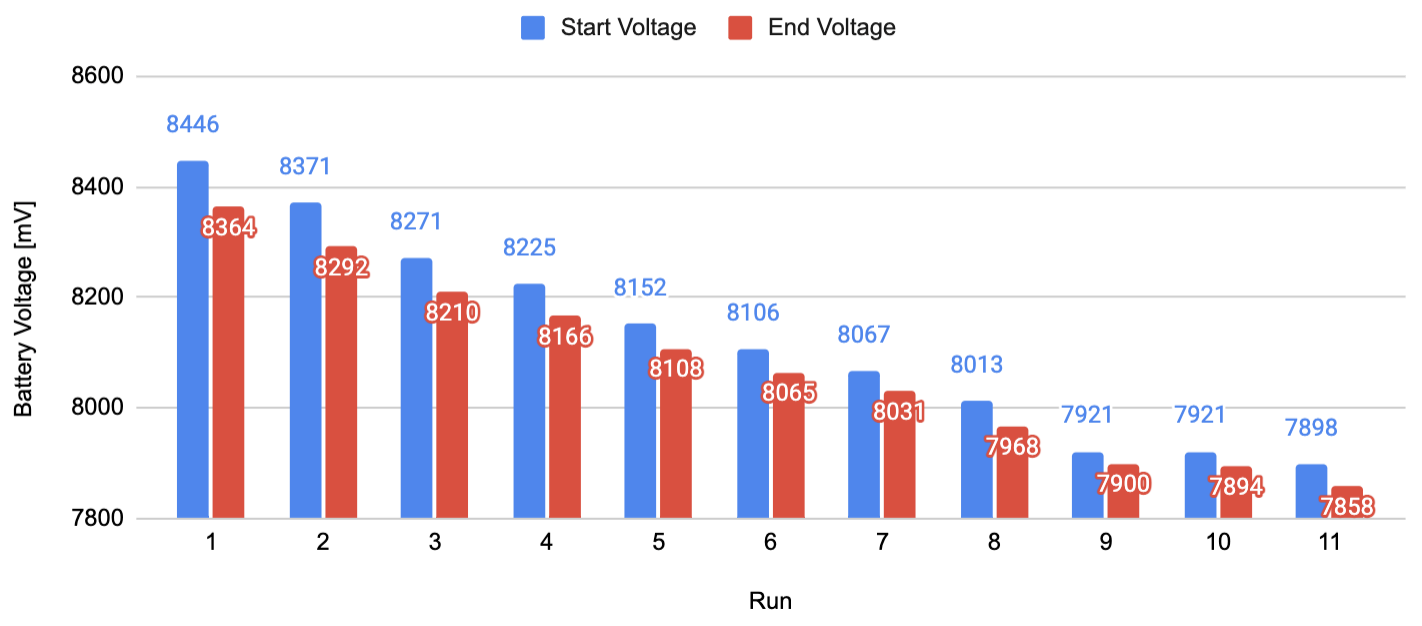
\includegraphics[width=\textwidth]{resources/turning-power.png}
    \caption{\TurnRob~- Comparison of start and end battery voltage per run}
    \label{fig:turning-power}
\end{figure}

The chart in Figure \ref{fig:turning-intersection-times} shows the average times required to scan and navigate each intersection type described in Figure \ref{fig:intersection_types}. The robot requires the most time to complete “dead end” intersections and the least for “right \& straight” and “straight” intersections.

\begin{figure}[!hbt]
    \centering
    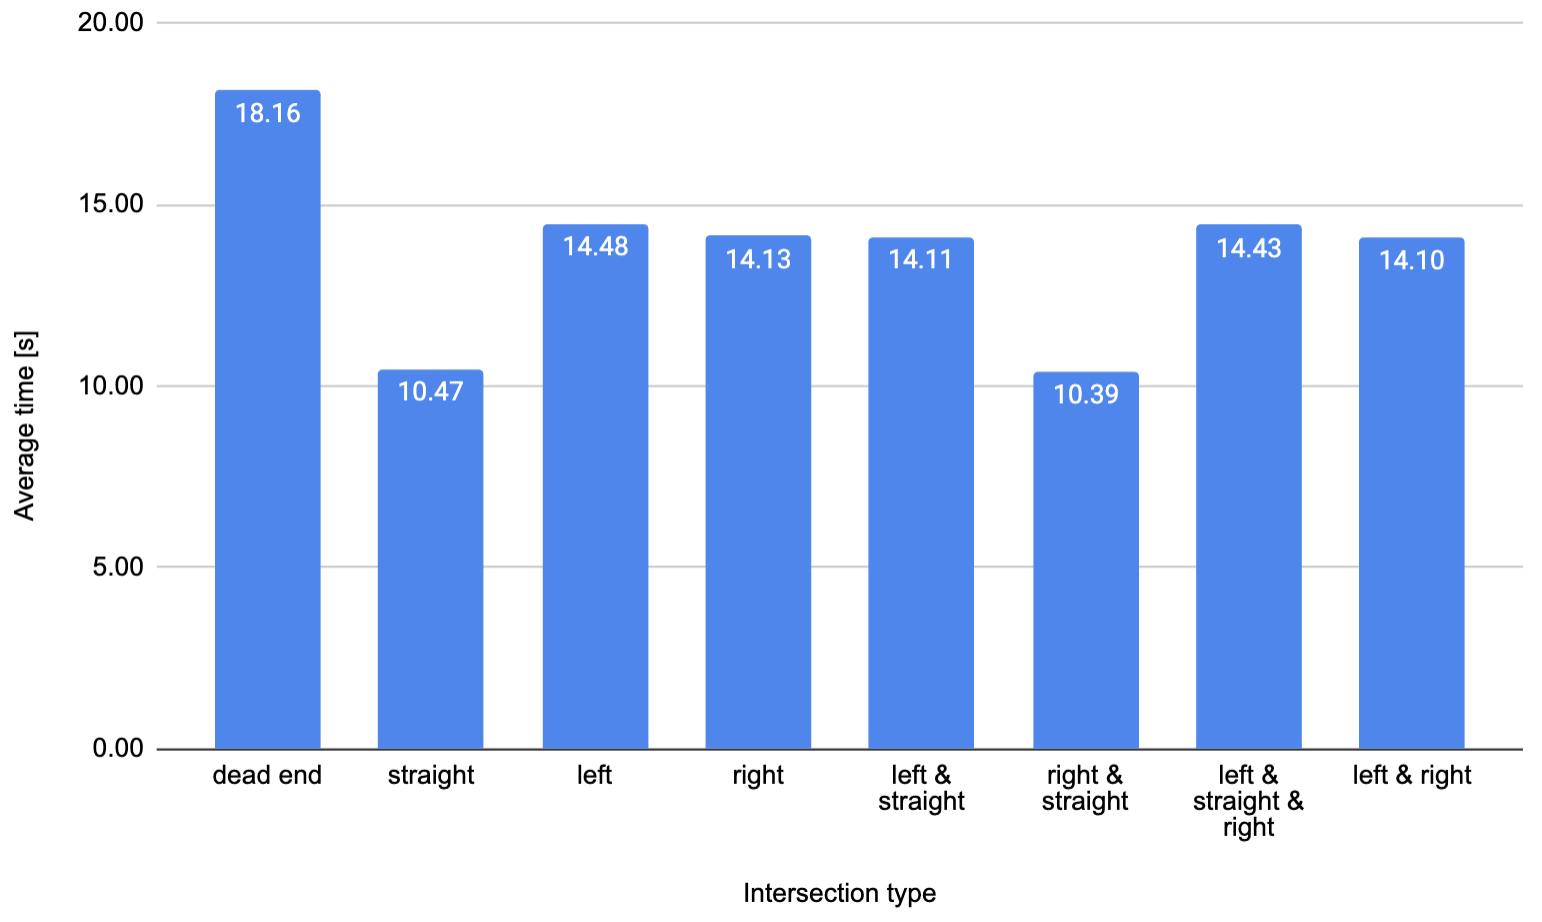
\includegraphics[width=\textwidth]{resources/turning-intersection-times.png}
    \caption{\TurnRob~- Average time per intersection type}
    \label{fig:turning-intersection-times}
\end{figure}

\subsubsection{Discussion} \label{sec:turning_discussion}

From the results, it is clear that also this robot configuration has consistent time in navigating through the maze, indicated by the relatively low standard deviation of 9.287. The deviations in time required for realignments are denoted by the standard deviation of 8.094 and have the same origin as the robot with the fixed sensor. Further explanation of why this deviation occurs can be found in Section \ref{sec:fixed_discussion}.

The time this robot spends on the line was calculated the same way as for \FixRob. Again, it was found that the average time spent on the line between intersections \#13 and \#14 was 10.45 seconds, and the average time spent on all other individual lines between intersections was only 2.55 seconds. This difference is present because the detection of the end of the maze is relatively slow, as already described for \FixRob in Section \ref{sec:fixed_discussion}.

For this robot, it is possible to detect a trend in the difference in battery voltage before and after each run by looking at the chart in Figure \ref{fig:turning-power}. The voltage drops steeply during the first runs because NiMH batteries' voltage also drops sharply at the beginning and then flats out. However, it can be seen in the graph that the last four measurements seem to be inaccurate, as it is expected that the consumed voltage becomes more and more constant as the voltage of the battery drops.

The results of the measurements of the average time required per intersection type in Figure \ref{fig:turning-intersection-times} show three groups characterised by very similar averages. The first group includes intersections where the robot continues driving \textit{straight}, averaging between 10.39 and 10.47 seconds. The second group contains intersections where the robot turns \textit{right} or \textit{left} and is recognised by an average between 14.11 and 14.48 seconds. The last group contains the \textit{dead end}, which takes 18.16 seconds on average.

The data show that \textit{dead ends} take the longest to scan and navigate. This is because the robot first turns the colour sensor to scan if there is a \textit{left} or \textit{straight} path available and then needs to turn 180 degrees to drive \textit{back} and exit the \textit{dead end}. Since the robot has to turn the farthest here to realign with the path, this intersection type takes the most time to navigate.

Intersections where the robot finally drives \textit{straight} are the fastest ones to complete as the robot directly continues driving forward after the scan is complete and does not need to turn.

As expected, the results show that the robot required the same amount of time for both \textit{left} and \textit{right} turns. This outcome is because the robot first scans for potential \textit{left} and \textit{straight} paths and then, depending on the result, turns 90 degrees to the \textit{left} or \textit{right} to align with the upcoming path. Since the scanning process is always the same and turning 90 degrees to the \textit{left} or \textit{right} takes up the same amount of time, the average \textit{left} and \textit{right} turns at intersections are the same.


\subsection{FixRob vs. TurnRob: Intersection time results}\label{sec:fixrob_vs_turnrob}

This section presents data that compares \FixRob and \TurnRob in terms of the time it takes them to scan and navigate through the eight intersection types represented in Figure \ref{fig:intersection_types}. These results are discussed in Section \ref{sec:discussion_intersections}.

Time differences at intersections were the greatest compared to time spent realigning or on the paths(see Figure \ref{tab:one_fixed_results} and \ref{tab:one_turning_results}). Table \ref{tab:combined_intersection_times} unifies the data from Figure \ref{fig:fixed-intersection-times} and Figure \ref{fig:turning-intersection-times} and shows the difference in the time the two robots require to complete the different intersection types in seconds and percentage. The data show that \FixRob is faster only at intersections where it finally takes the \textit{left} path. In contrast, \TurnRob is faster than \FixRob at all other intersection types, where the robot ultimately drives \textit{straight}, \textit{right} or \textit{back}.

\begin{table}[h!]
\caption{Comparison of both robot's intersection types statistics. (\textit{Path taken} is \textbf{L}eft, \textbf{S}traight, \textbf{R}ight, \textbf{B}ack from the perspective where the robot arrived at the intersection.)}
\label{tab:combined_intersection_times}
\resizebox{\textwidth}{!}{
\begin{tabular}{clcccc}
\hline
 \multicolumn{2}{c}{Intersection} & & \multicolumn{2}{c}{\FixRob compared to \TurnRob (Avg.)} \\ \cline{1-2} \cline{4-5}
%\hline
Id &
  Description &
    Path taken &
  \multicolumn{1}{c}{Single intersection{[}s{]}} &
  \multicolumn{1}{c}{Percentage{[}\%{]}} \\ \hline 
1     & dead end                  & B & $+$4.54  & $+$25.00 \\
2     & straight                  & S & $+$4.08  & $+$38.97 \\
3     & left                      & L & $-$3.46  & $-$23.92 \\
4     & right                     & R & $+$4.58  & $+$32.42 \\
5     & left \& straight          & L & $-$3.24  & $-$22.94 \\
6     & right \& straight         & S & $+$4.00  & $+$38.52 \\
7     & left \& straight \& right & L & $-$3.55  & $-$24.61 \\
8     & left \& right             & L & $-$3.07  & $-$21.80 \\ \hline
Sum   &                           &   & $+$3.88  & $+$3.52  \\ \hline
\end{tabular}
}
\end{table}


The sum of the time required for \TurnRob to complete each of the eight intersection types is 3.88 seconds (3.52\%) less than that of \FixRob. Therefore, for a maze with exactly one intersection per intersection type, \TurnRob is expected to take 3.88 seconds (3.52\%) less to navigate through the intersections than \FixRob.


According to these calculations, the time difference between the two robots for intersection scanning and navigation for the entire test maze is estimated to be 3.85 seconds. The average total intersection time for \FixRob is 243.17 seconds and 240.20 seconds for \TurnRob.